\appendix

\chapter{Reproducibility}

\section{Implementation Details}
All our experiment are conducted using Python 3.12.7 and the version 1.2.6 of compressAI (see requirements file for other libraries version). We used an Anaconda virtual environment on the Télécom Paris GPU cluster which provides the processign power to perform our trainings and testings. All the code for our experiments is available on the following GitHub repository: \url{}

We also need to adress how we obtain the measures of Section \ref{application_resource_contrained_platforms}. Utilizing PyTorch properties, we use the following functions to compute the number of parameters and the memory footprint of the models:

\begin{pythonCode}
def model_nb_param(model):
    return sum(p.numel() for p in model.parameters()) / 1_000_000 # Convert to M parameters


def model_memory_size(model):
    param_size = 0
    for param in model.parameters():
        param_size += param.nelement() * param.element_size()
    buffer_size = 0
    for buffer in model.buffers():
        buffer_size += buffer.nelement() * buffer.element_size()

    size_all_mb = (param_size + buffer_size) / 1024**2 # Convert to MB
    return size_all_mb
\end{pythonCode}

\acrshort{flop}s are measured once per model using the \textsf{FlopCountAnalysis} from the fvcore library. We use two liraries to compute the inference time and energy consumption of the models: pynvml and zeus. By iterating 50 times through the test dataset images loaded on the same Nvidia RTX 3090 GPU beforehand, we are able to achieve meaningful average values per frame. Both libraries present similar results and we ultimatly chose the zeus library for our final results. The value of inference time per frame is used to compute the model througput.

In Section \ref{application_resource_contrained_platforms}, we use the PIL Python library to convert images from the Kodak dataset to JPEG-2000, JPEG and Webp. We follow the same method as for evaluating \acrshort{nn}s.

\chapter{Figures}

\begin{figure}
    \centering
    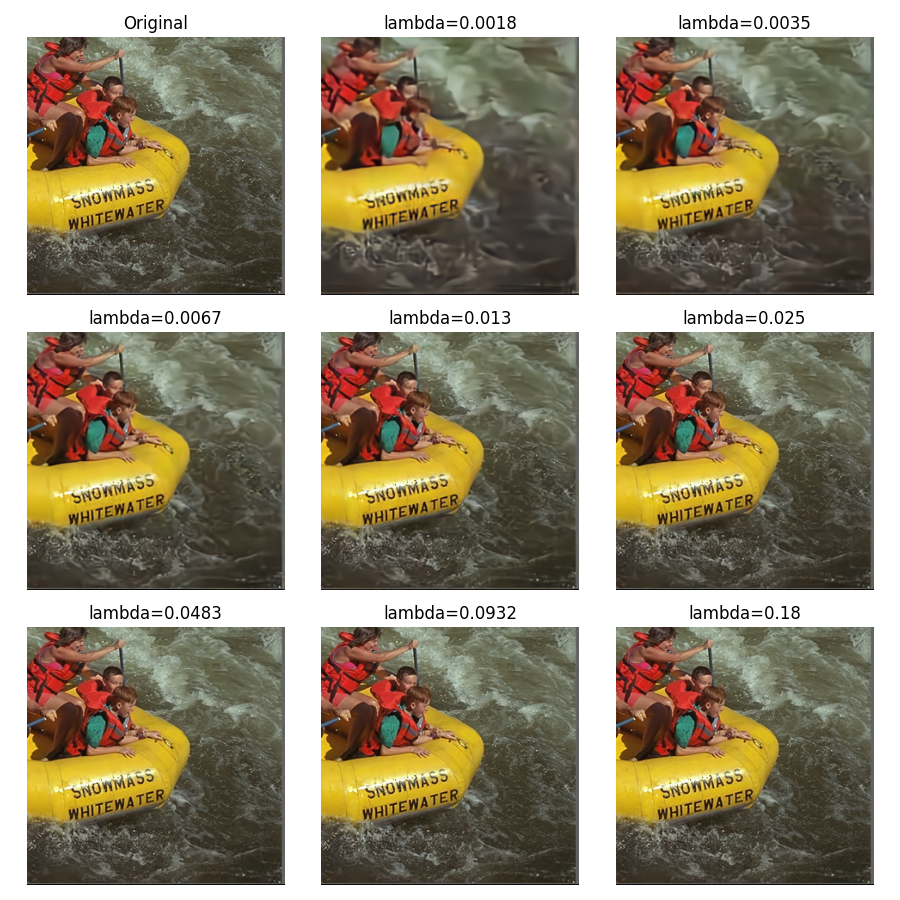
\includegraphics[width=15cm]{../img/bdpsnr_kodak_14_pretrained.png}
    \caption[econstruction results on image 14 of the Kodak dataset for different RD tradeoffs (pre-trained models).]{econstruction results on image 14 of the Kodak dataset for different RD tradeoffs (pre-trained models).}
    \label{appendix:bdpsnr_1:a}
\end{figure}

\begin{figure}
    \centering
    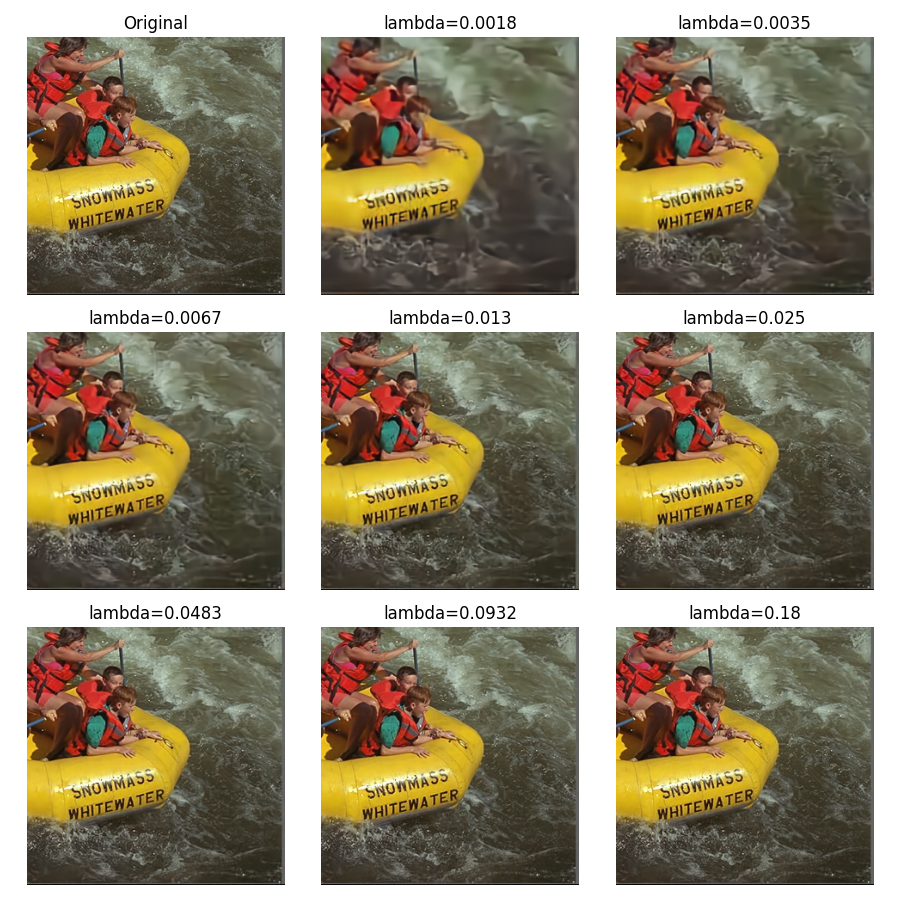
\includegraphics[width=15cm]{../img/bdpsnr_kodak_14.png}
    \caption[econstruction results on image 14 of the Kodak dataset for different RD tradeoffs (our models).]{econstruction results on image 14 of the Kodak dataset for different RD tradeoffs (our models).}
    \label{appendix:bdpsnr_1:b}
\end{figure}

\begin{figure}
    \centering
    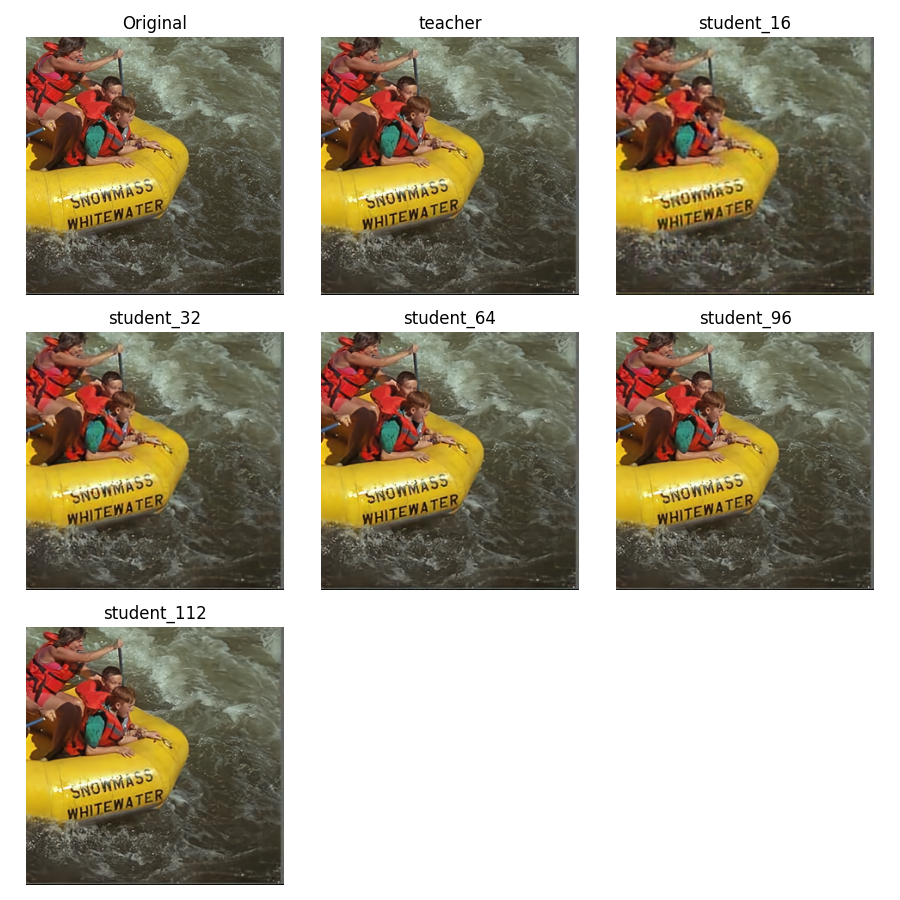
\includegraphics[width=15cm]{../img/kd_ae_kodak_14.png}
    \caption[Evaluation on the Kodak dataset of the scale hyperprior student models trained for image reconstruction: reconstruction results on image 14 of the Kodak dataset with teacher and student architectures.]{Evaluation on the Kodak dataset of the scale hyperprior student models trained for image reconstruction: reconstruction results on image 14 of the Kodak dataset with teacher and student architectures.}
    \label{appendix:kd_ae_1:a}
\end{figure}

\begin{figure}
    \centering
    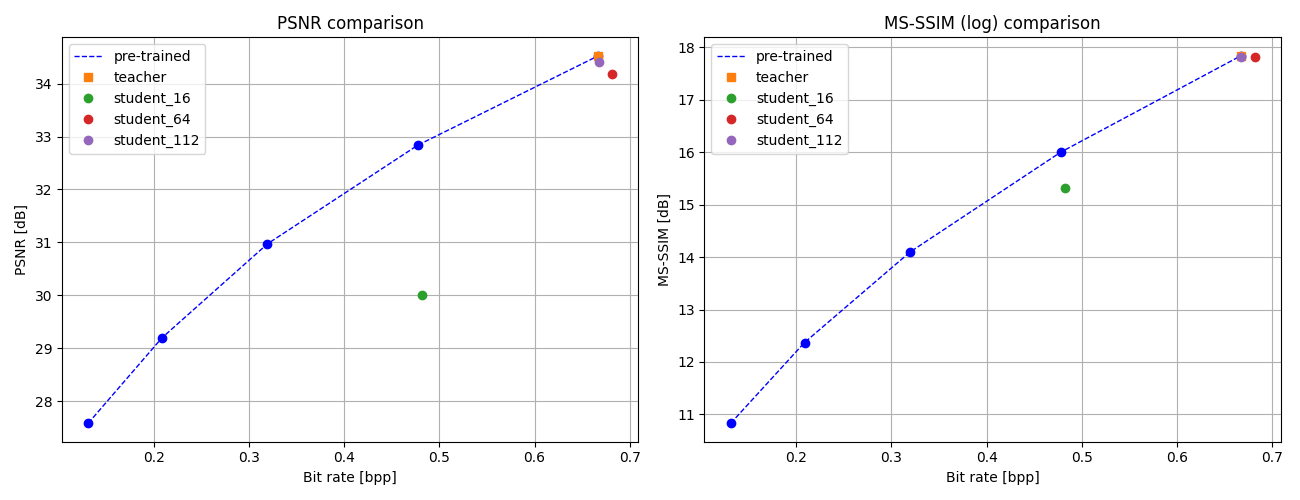
\includegraphics[width=15cm]{../img/kd_lic_rd_channels_kld.png}
    \caption[Average \acrshort{rd} curve on the Kodak dataset for students with different number of channels and Kullback-Leibler divergence loss on the latent space.]{Average \acrshort{rd} curve on the Kodak dataset for students with different number of channels and Kullback-Leibler divergence loss on the latent space.}
    \label{appendix:kd_lic_1_kld}
\end{figure}

\begin{figure}
    \centering
    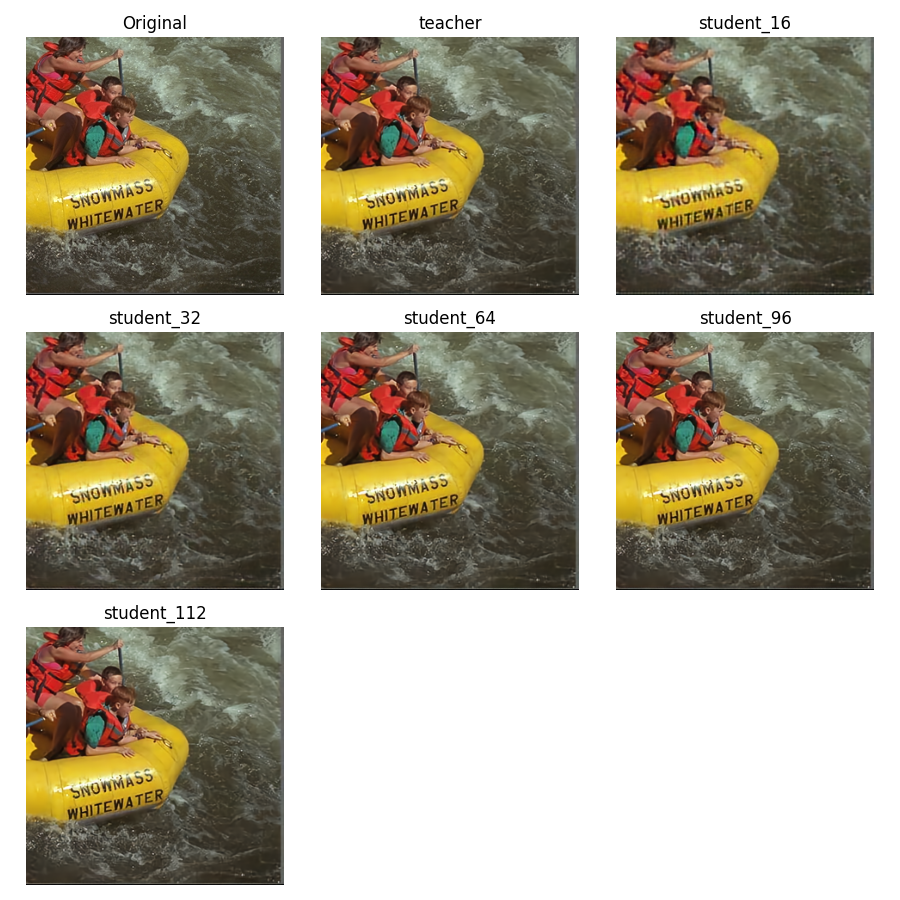
\includegraphics[width=15cm]{../img/kd_lic_kodak_14.png}
    \caption[Evaluation on the Kodak dataset of the scale hyperprior student models trained for image compression: reconstruction results on image 14 of the Kodak dataset with teacher and student architectures.]{Evaluation on the Kodak dataset of the scale hyperprior student models trained for image compression: reconstruction results on image 14 of the Kodak dataset with teacher and student architectures.}
    \label{appendix:kd_lic_2:a}
\end{figure}

\begin{figure}
    \centering
    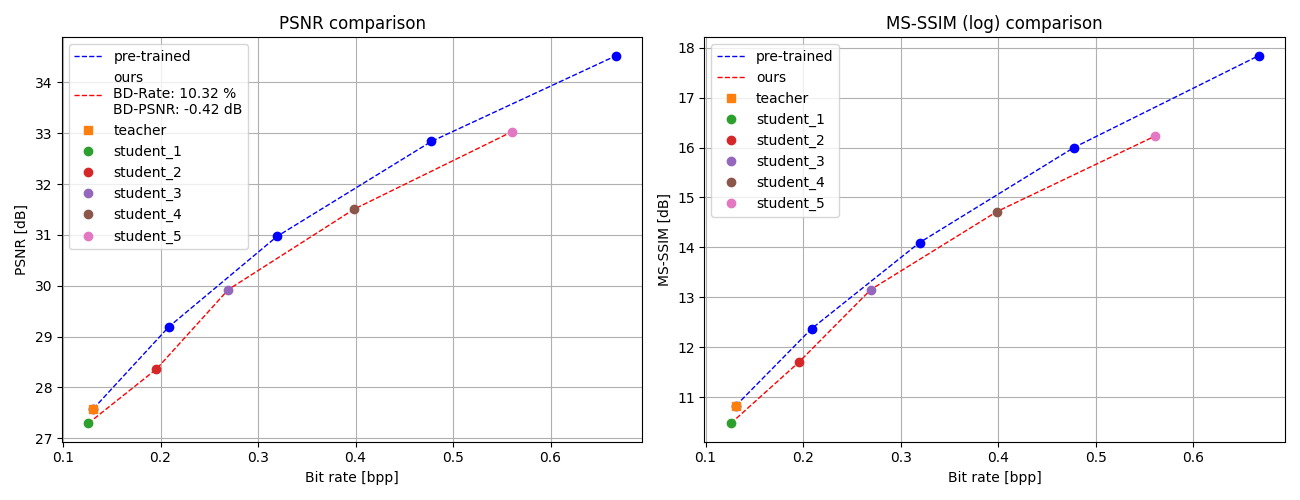
\includegraphics[width=15cm]{../img/kd_lic_rd_lambda_2.png}
    \caption[Average \acrshort{rd} curve on the Kodak dataset for students with different \acrshort{rd} tradeoffs and a teacher focusing on minimising bit rate.]{Average \acrshort{rd} curve on the Kodak dataset for students with different \acrshort{rd} tradeoffs and a teacher focusing on minimising bit rate.}
    \label{appendix:kd_lic_4_bis}
\end{figure}
% Use 289751, 295889, 289745, 296544, 289742

\begin{figure}
    \centering
    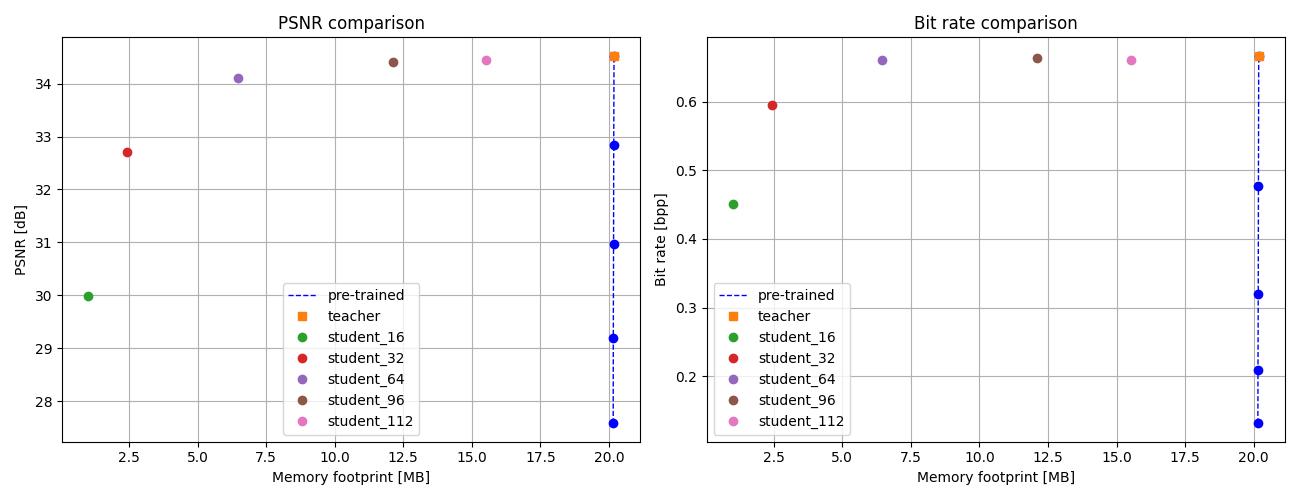
\includegraphics[width=15cm]{../img/kd_lic_memory.png}
    \caption[\acrshort{psnr} and bit rate on the Kodak dataset according to students memory footprint.]{\acrshort{psnr} and bit rate on the Kodak dataset according to students memory footprint.}
    \label{appendix:kd_lic_memory}
\end{figure}

\begin{figure}
    \centering
    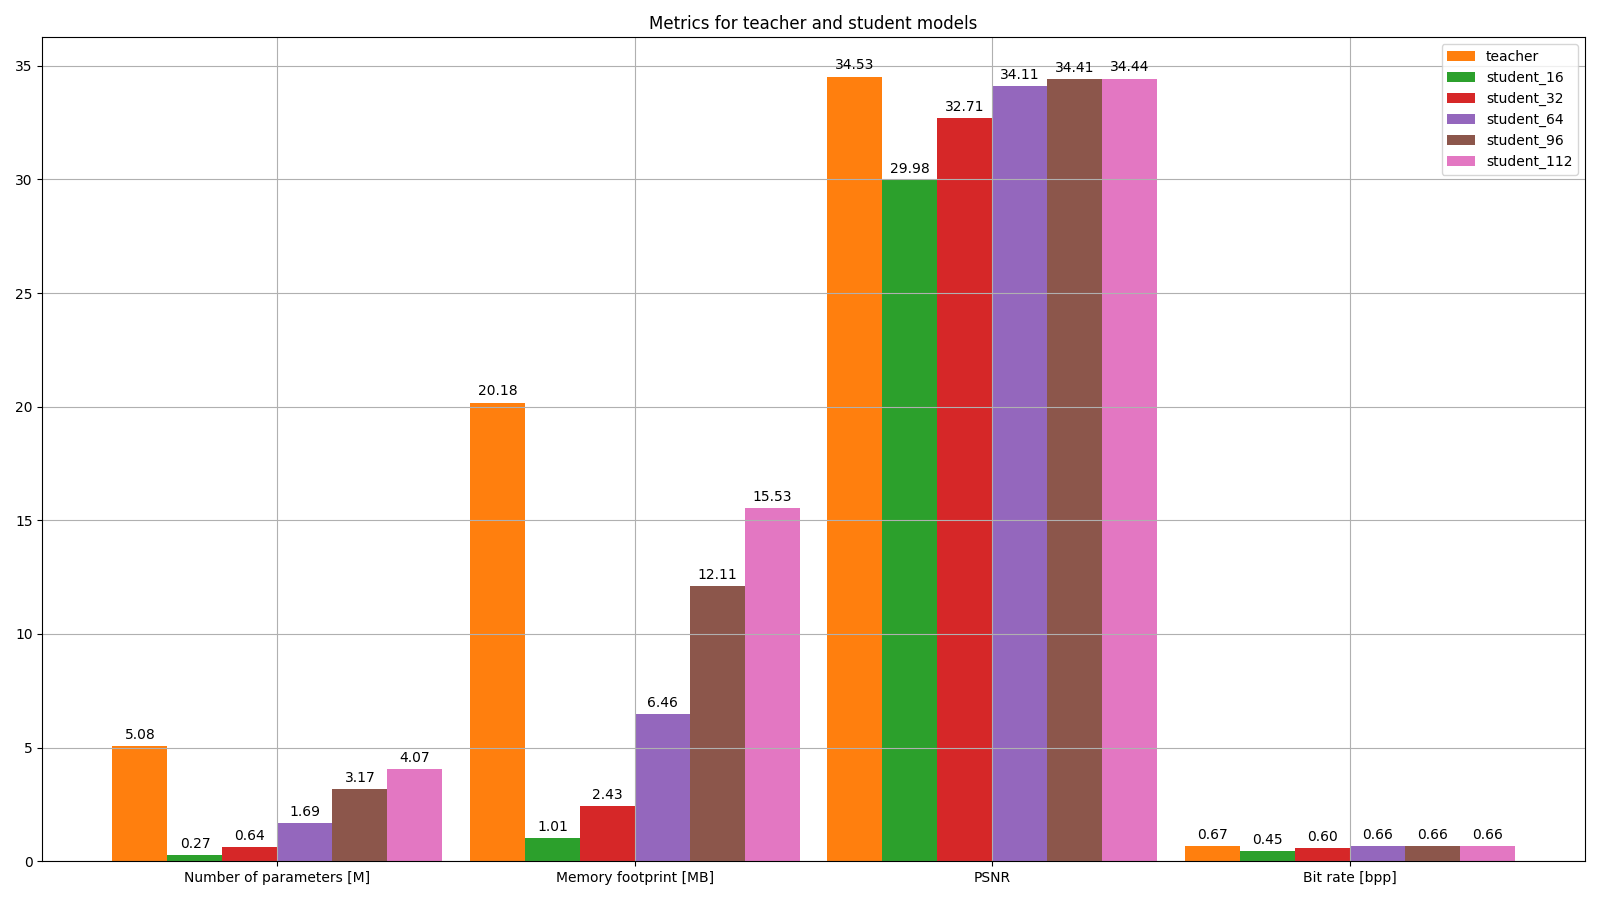
\includegraphics[width=15cm]{../img/kd_lic_bar_size.png}
    \caption[Number of parameters, memory footprint, \acrshort{psnr} and bit rate bar chart for teacher and student models.]{Number of parameters, memory footprint, \acrshort{psnr} and bit rate bar chart for teacher and student models.}
    \label{appendix:kd_lic_bar_size}
\end{figure}

\begin{figure}
    \centering
    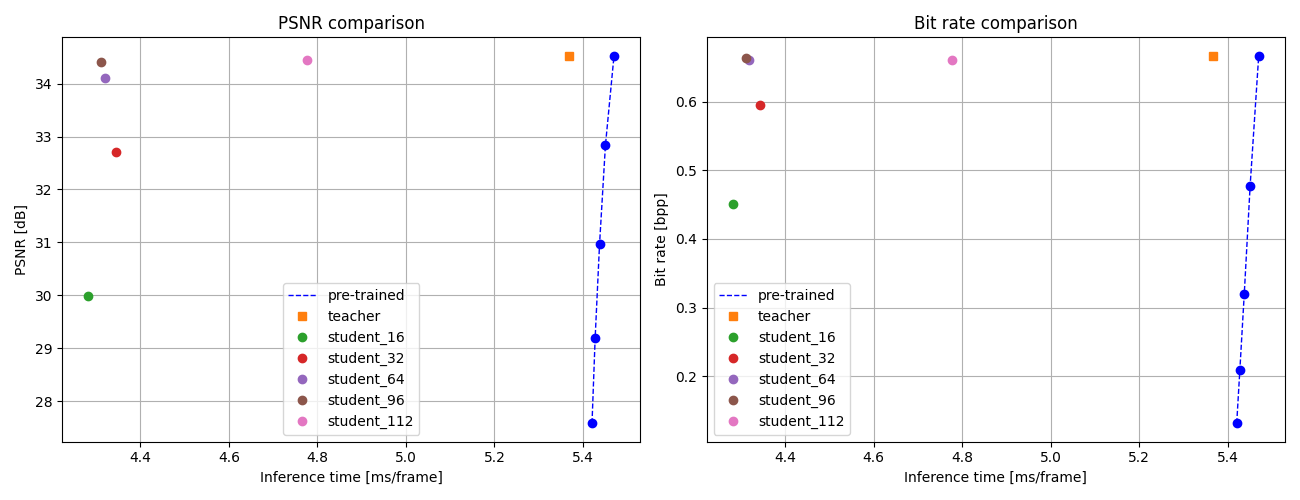
\includegraphics[width=15cm]{../img/kd_lic_time.png}
    \caption[\acrshort{psnr} and bit rate on the Kodak dataset according to students inference time.]{\acrshort{psnr} and bit rate on the Kodak dataset according to students inference time.}
    \label{appendix:kd_lic_time}
\end{figure}

\begin{figure}
    \centering
    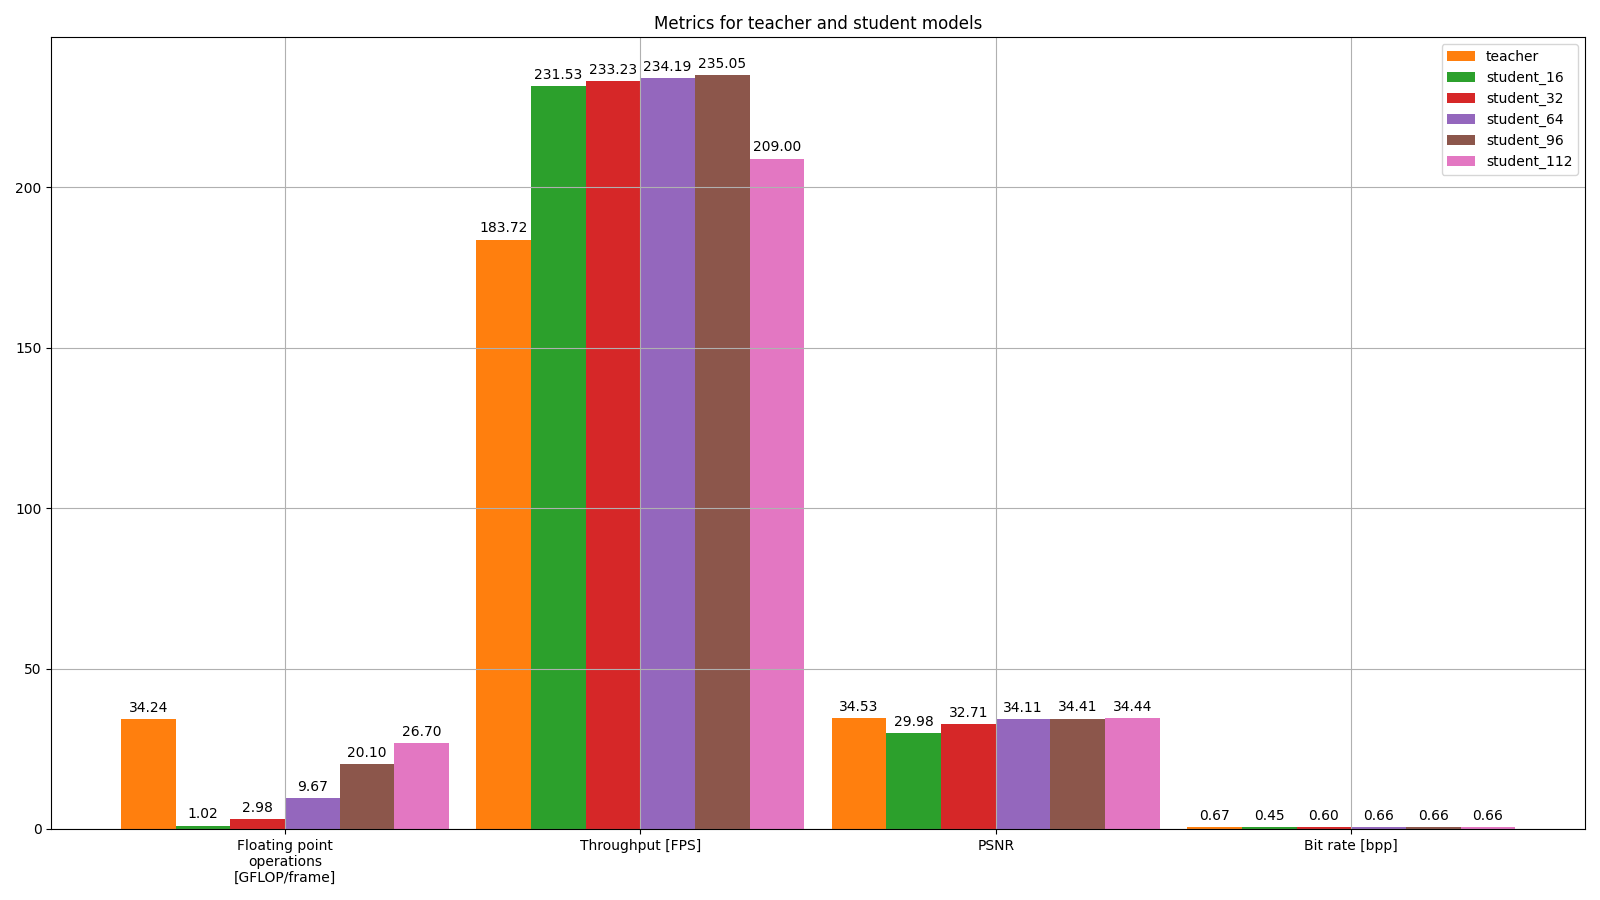
\includegraphics[width=15cm]{../img/kd_lic_bar_compute.png}
    \caption[\acrshort{flop}s, throughput, \acrshort{psnr} and bit rate bar chart for teacher and student models.]{\acrshort{flop}s, throughput, \acrshort{psnr} and bit rate bar chart for teacher and student models.}
    \label{appendix:kd_lic_bar_compute}
\end{figure}

\begin{figure}
    \centering
    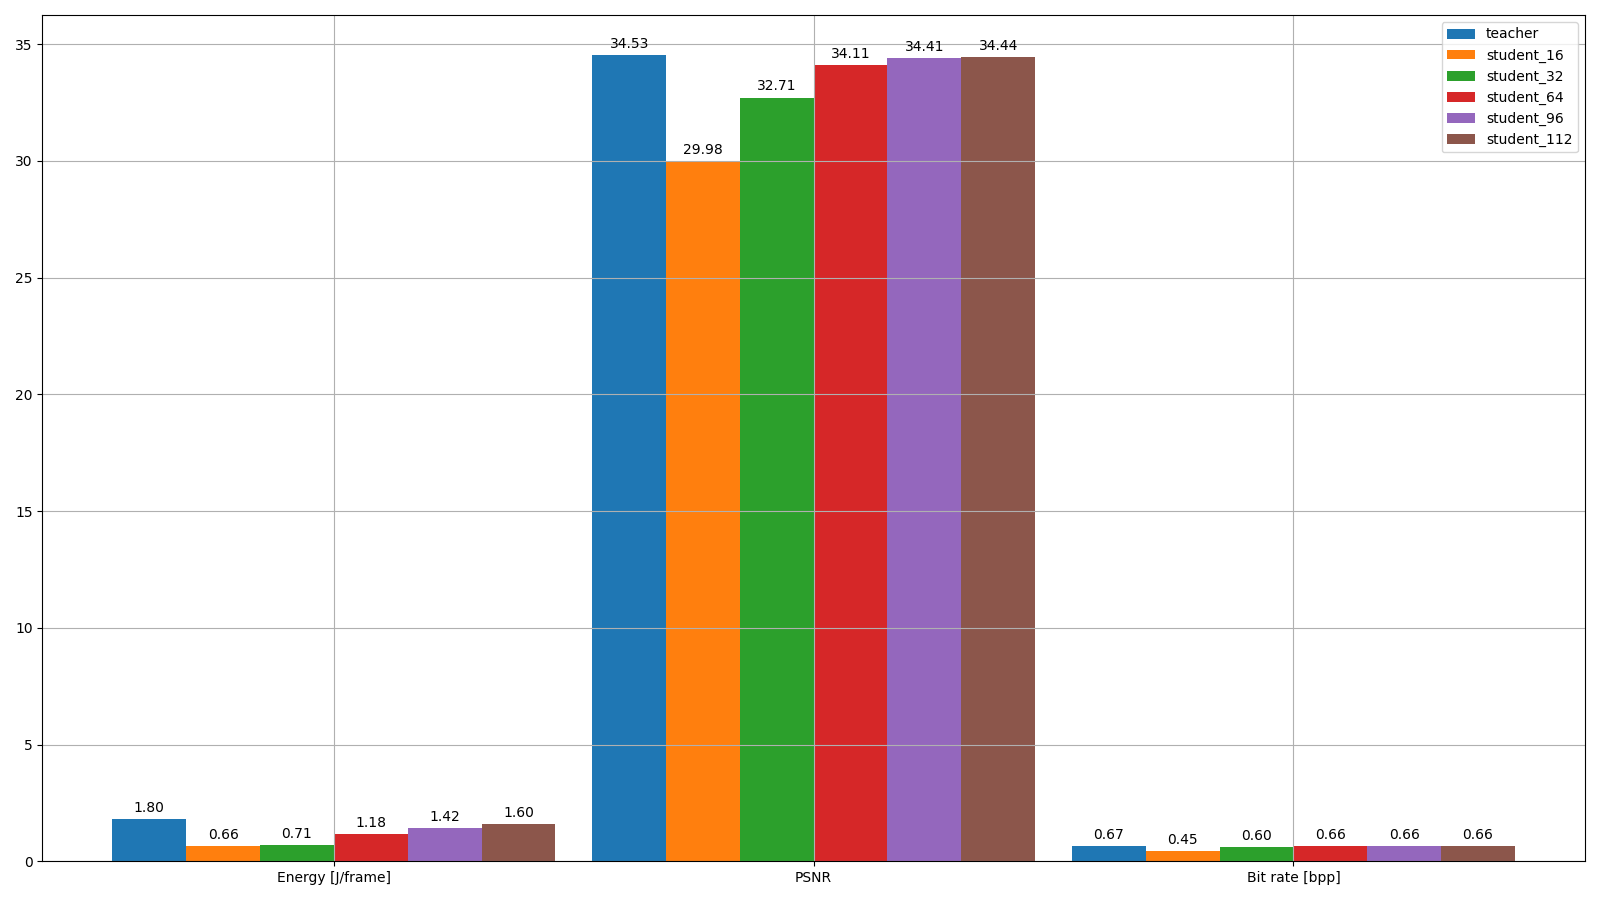
\includegraphics[width=15cm]{../img/kd_lic_bar_energy.png}
    \caption[Consumed energy, \acrshort{psnr} and bit rate bar chart for teacher and student models.]{Consumed energy, \acrshort{psnr} and bit rate bar chart for teacher and student models.}
    \label{appendix:kd_lic_bar_energy}
\end{figure}

\begin{sidewaystable}[]
    \centering
    \begin{tabular}{|c|c|lr|lr|lr|lr|lr|lr|lr|}
        \hline
        Model                     & \begin{tabular}[c]{@{}c@{}}Number\\ of channels\end{tabular} & \multicolumn{2}{c|}{\begin{tabular}[c]{@{}c@{}}Number of\\ parameters {[}M{]}\end{tabular}} & \multicolumn{2}{c|}{\begin{tabular}[c]{@{}c@{}}Memory\\ footprint {[}MB{]}\end{tabular}} & \multicolumn{2}{c|}{\begin{tabular}[c]{@{}c@{}}Floating point\\ operations\\ {[}GFLOP/frame{]}\end{tabular}} & \multicolumn{2}{c|}{\begin{tabular}[c]{@{}c@{}}Throughput\\ {[}FPS{]}\end{tabular}} & \multicolumn{2}{c|}{\begin{tabular}[c]{@{}c@{}}Energy\\ {[}mJ/frame{]}\end{tabular}} & \multicolumn{2}{c|}{PSNR}               & \multicolumn{2}{c|}{\begin{tabular}[c]{@{}c@{}}Bit rate\\ {[}bpp{]}\end{tabular}}      \\ \hline
        Teacher                   & 128                        & {\color[HTML]{656565} }                                  & 5.08                         & {\color[HTML]{656565} }                                  & 20.18                        & {\color[HTML]{656565} }                                  & 34.24                        & {\color[HTML]{656565} }                                  & 184.20                         & {\color[HTML]{656565} }                                  & 1767.85                         & {\color[HTML]{656565} }                                 & 34.53                         & {\color[HTML]{656565} }                                 & 0.67                         \\ \hline
                                  & 112                        & {\color[HTML]{656565} -19.77 \%}                         & 4.07                         & {\color[HTML]{656565} -23.03 \%}                         & 15.53                        & {\color[HTML]{656565} -22.01 \%}                         & 26.70                        & {\color[HTML]{656565} +13.47 \%}                         & 209.01                         & {\color[HTML]{656565} -9.47 \%}                          & 1600.41                         & {\color[HTML]{656565} -0.26 \%}                         & 34.44                         & {\color[HTML]{656565} -1.03 \%}                         & 0.66                         \\ \cline{2-16} 
                                  & 96                         & {\color[HTML]{656565} -37.47 \%}                         & 3.17                         & {\color[HTML]{656565} -40.01 \%}                         & 12.11                        & {\color[HTML]{656565} -41.31 \%}                         & 20.10                        & {\color[HTML]{656565} +25.74 \%}                         & 231.61                         & {\color[HTML]{656565} -19.88 \%}                         & 1416.34                         & {\color[HTML]{656565} -0.33 \%}                         & 34.41                         & {\color[HTML]{656565} -0.58 \%}                         & 0.66                         \\ \cline{2-16} 
                                  & \cellcolor[HTML]{EFEFEF}64 & \cellcolor[HTML]{EFEFEF}{\color[HTML]{656565} -66.62 \%} & \cellcolor[HTML]{EFEFEF}1.69 & \cellcolor[HTML]{EFEFEF}{\color[HTML]{656565} -67.98 \%} & \cellcolor[HTML]{EFEFEF}6.46 & \cellcolor[HTML]{EFEFEF}{\color[HTML]{656565} -71.75 \%} & \cellcolor[HTML]{EFEFEF}9.67 & \cellcolor[HTML]{EFEFEF}{\color[HTML]{656565} +26.20 \%} & \cellcolor[HTML]{EFEFEF}232.47 & \cellcolor[HTML]{EFEFEF}{\color[HTML]{656565} -34.15 \%} & \cellcolor[HTML]{EFEFEF}1164.17 & \cellcolor[HTML]{EFEFEF}{\color[HTML]{656565} -1.21 \%} & \cellcolor[HTML]{EFEFEF}34.11 & \cellcolor[HTML]{EFEFEF}{\color[HTML]{656565} -0.91 \%} & \cellcolor[HTML]{EFEFEF}0.66 \\ \cline{2-16} 
                                  & 32                         & {\color[HTML]{656565} -87.46 \%}                         & 0.64                         & {\color[HTML]{656565} -87.97 \%}                         & 2.43                         & {\color[HTML]{656565} -91.31 \%}                         & 2.98                         & {\color[HTML]{656565} +25.89 \%}                         & 231.90                         & {\color[HTML]{656565} -60.45 \%}                         & 699.18                          & {\color[HTML]{656565} -5.25 \%}                         & 32.71                         & {\color[HTML]{656565} -10.73 \%}                        & 0.60                         \\ \cline{2-16} 
        \multirow{-5}{*}{Student} & 16                         & {\color[HTML]{656565} -94.77 \%}                         & 0.27                         & {\color[HTML]{656565} -94.98 \%}                         & 1.01                         & {\color[HTML]{656565} -97.01 \%}                         & 1.02                         & {\color[HTML]{656565} +26.83 \%}                         & 233.63                         & {\color[HTML]{656565} -61.28 \%}                         & 684.45                          & {\color[HTML]{656565} -13.17 \%}                        & 29.98                         & {\color[HTML]{656565} -32.44 \%}                        & 0.45                         \\ \hline
    \end{tabular}
    \caption[Number of parameters, memory footprint, \acrshort{flop}s, throughput, consumed energy, \acrshort{psnr} and bit rate for teacher and student models.]{Number of parameters, memory footprint, \acrshort{flop}s, throughput, consumed energy, \acrshort{psnr} and bit rate for teacher and student models.}
    \label{appendix:tab_resources}
\end{sidewaystable}

\begin{figure}
    \centering
    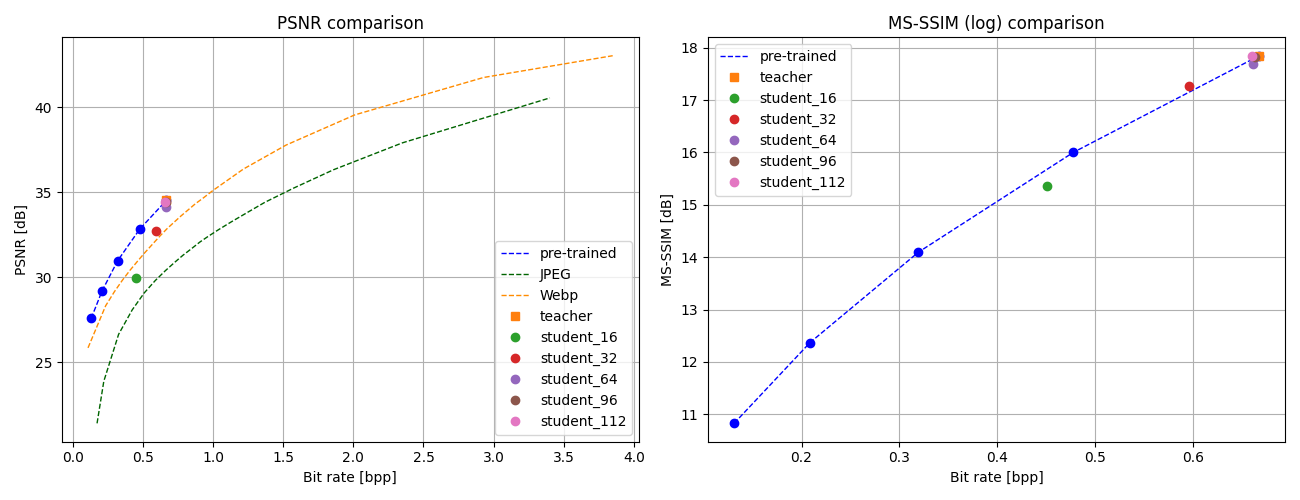
\includegraphics[width=15cm]{../img/codecs_rd.png}
    \caption[Average \acrshort{rd} curve on the Kodak dataset for students with different number of channels and codecs.]{Average \acrshort{rd} curve on the Kodak dataset for students with different number of channels and codecs.}
    \label{appendix:codecs_rd}
\end{figure}

\begin{figure}
    \centering
    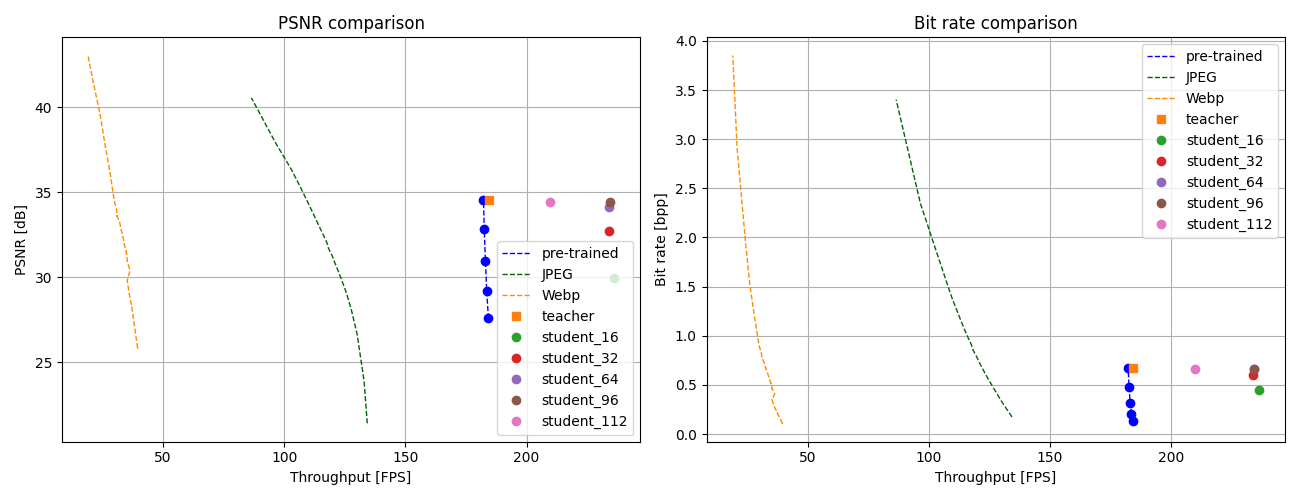
\includegraphics[width=15cm]{../img/codecs_fps.png}
    \caption[\acrshort{psnr} and bit rate on the Kodak dataset according to students and codecs throughput.]{\acrshort{psnr} and bit rate on the Kodak dataset according to students and codecs throughput.}
    \label{appendix:codecs_fps}
\end{figure}

\begin{figure}
    \centering
    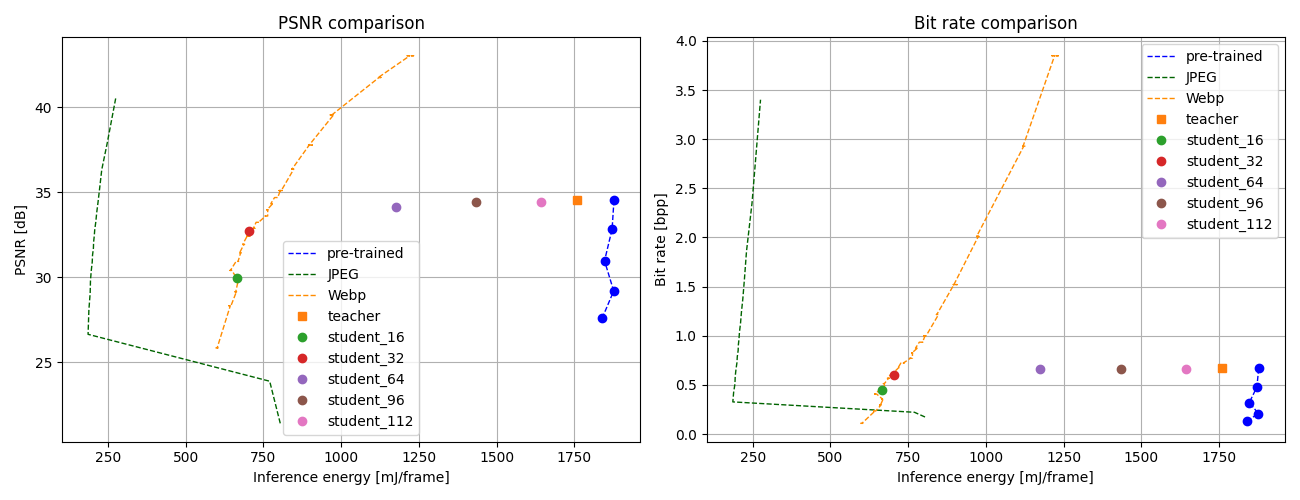
\includegraphics[width=15cm]{../img/codecs_energy.png}
    \caption[\acrshort{psnr} and bit rate on the Kodak dataset according to students and codecs consumed energy.]{\acrshort{psnr} and bit rate on the Kodak dataset according to students and codecs consumed energy.}
    \label{appendix:codecs_energy}
\end{figure}